\subsection{ERROR REDUCTION}

In this section, we discuss about the error in analysis of the images. In this sense,
we can see that, the targets have different forms; however, 
a $ROI$ ever will have a rectangular form, so that certain areas will be more important of identify inside of $ROI$.
In Fig. \ref{fig:erroridentified}, there are some areas close of edges that target not occupies; they are
considered like error areas.

\begin{figure}[H]
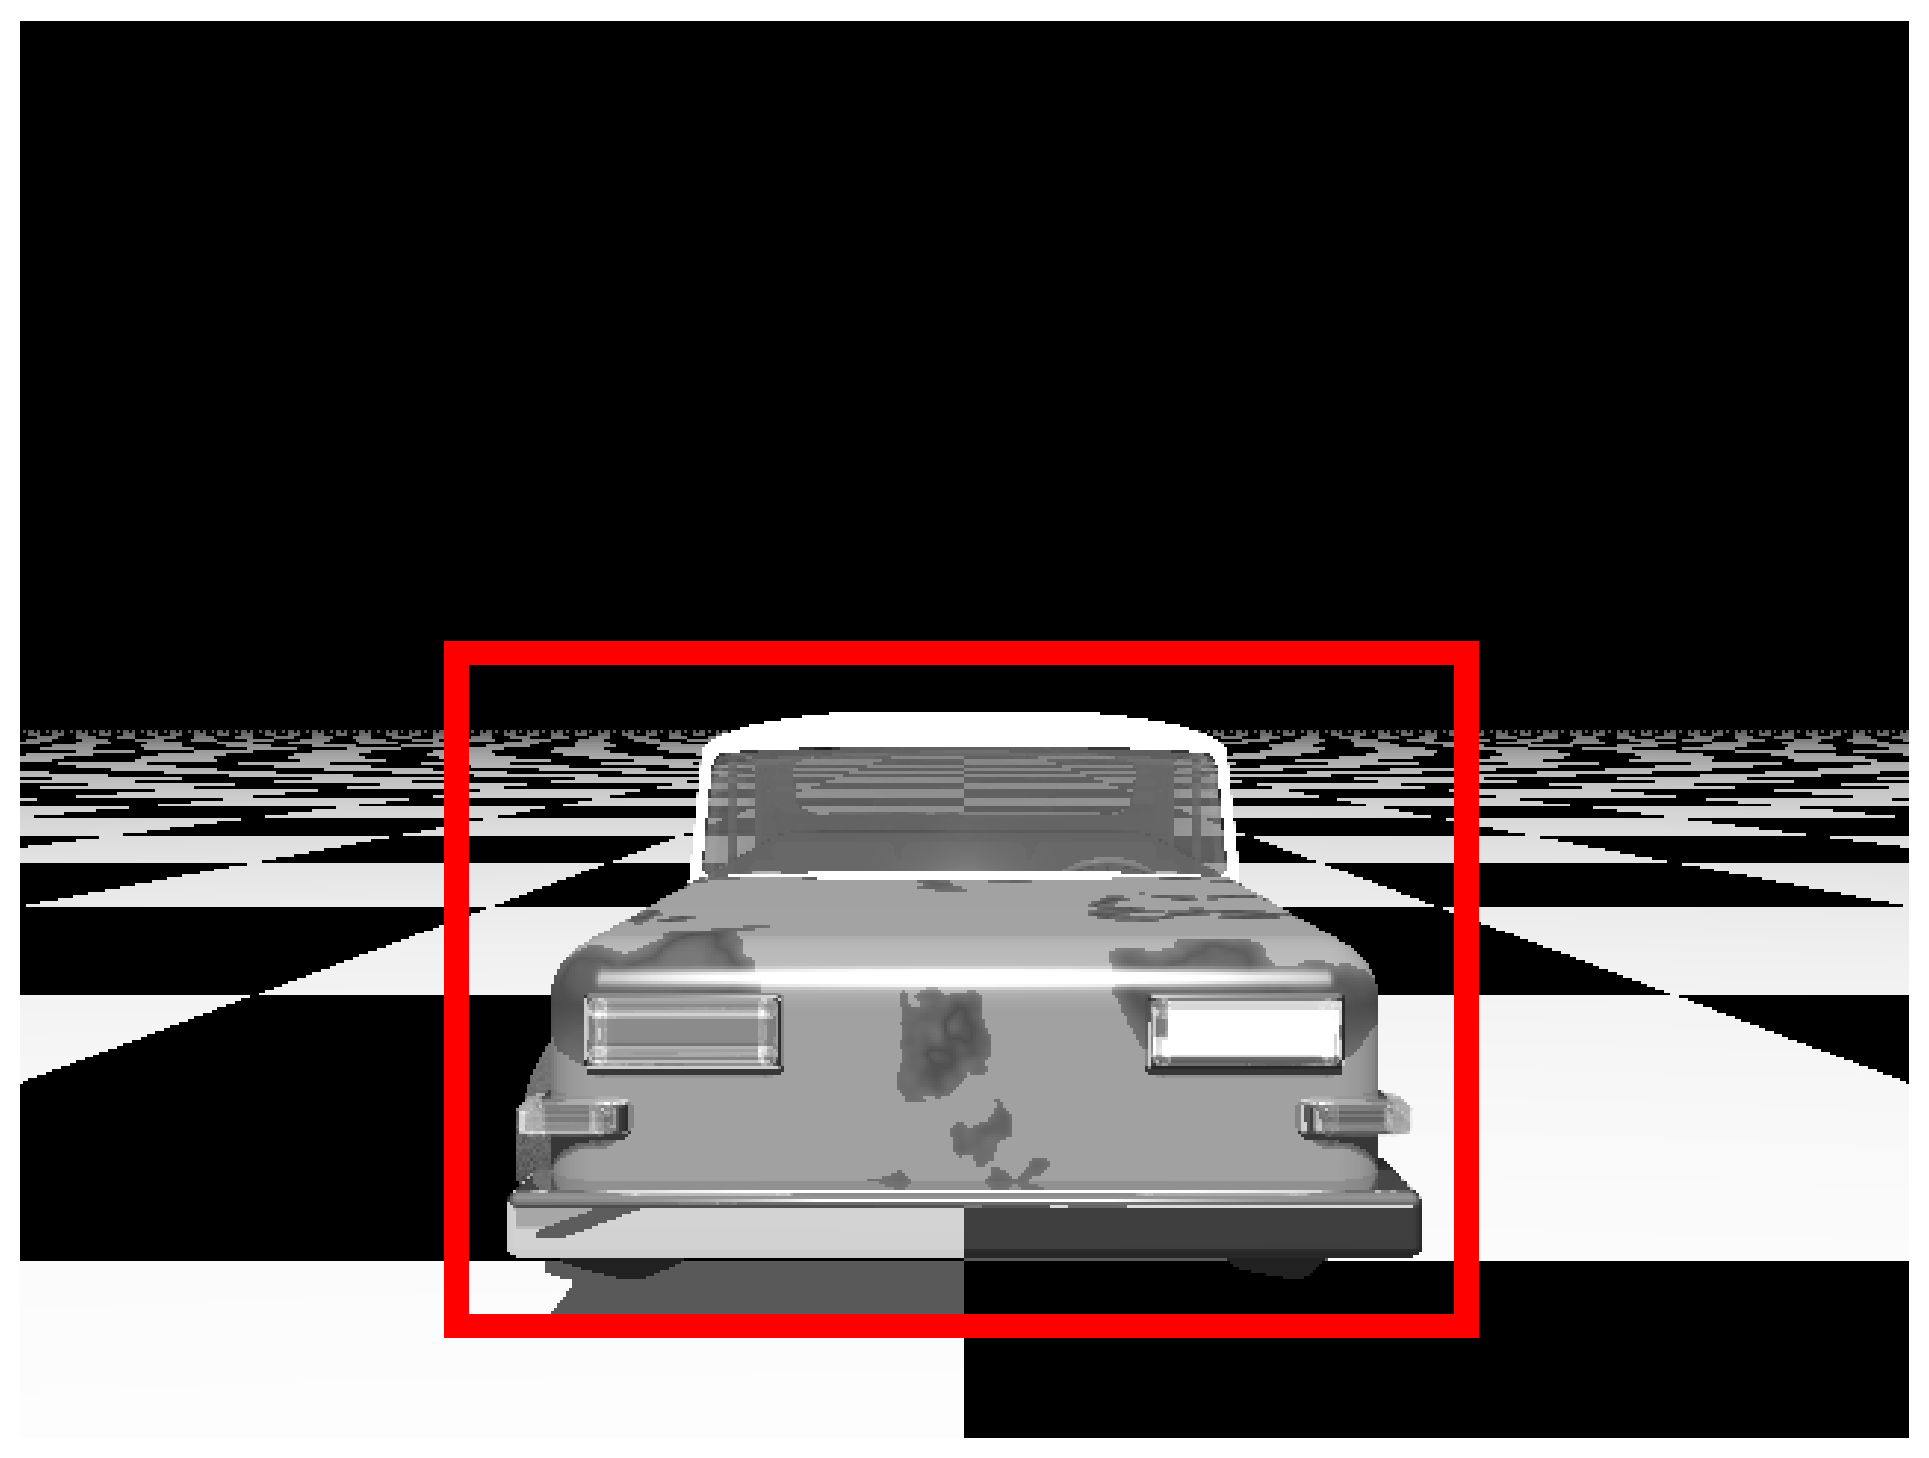
\includegraphics[width=\columnwidth]{images/imageError.eps}
\caption{Illustration of $ROI$ with error areas close of edge.}
\label{fig:erroridentified}
\end{figure}

By other side, two matrix with the same dimensions can be compared using $PCC$; 
this method of comparison doesn't generate data over if the frame are equals,
and yes over if the frames have a proportional behavior in the relation of your values. 
Thus, a high percentage of error area when compared with the target area 
may decrease the correlation level between frames, promoting the loss of the target. 
We decide solve this problem using a weighing matrix mask over the analyzed regions, 
before the calculus of $PCC$. This can be seen in the Fig. \ref{fig:errorpondered}.
\begin{figure}[H]
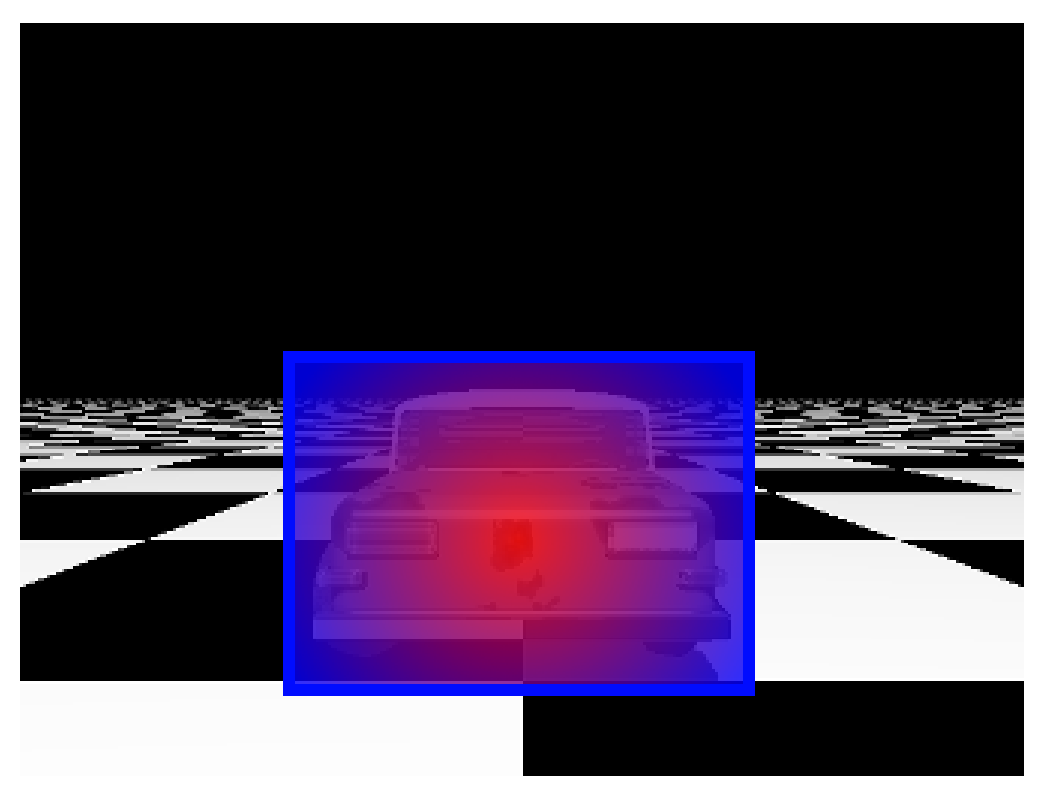
\includegraphics[width=\columnwidth]{images/imageErrorcontroled.eps}
\caption{Illustration of points of most importance (red) and points less importance (blue) in correlation.}
\label{fig:errorpondered}
\end{figure}
Where, points close of edge (in blue color) have less importance, 
points close of center of image (in red color), probably are on the target, and consequently
these points will have more importance. 

Thus, the $Q(x,y)$ value showed in the Eq. (\ref{eq:Q}), 
\begin{equation}\label{eq:Q}
 Q(x,y) = \sqrt{e^{ -\frac{|x-\mu_X|^3}{\sigma_X^3}-\frac{|y-\mu_Y|^3}{\sigma_Y^3}  }},
\end{equation}
represents a value, in the line $x$ and column $y$, on the weighing matrix mask $Q$,
where $\mu_X=H/2$, $\mu_Y=W/2$, $\sigma_X=H/3$ and $\sigma_Y=W/3$; being $H$ and $W$
the height and the width, respectively, in the analysis region.

Finally, similarly to seen in the Eq. (\ref{eq:PCC}), we multiply the matrix $Q$, 
element by element, over the analysis regions
$A$ and $B$ to calculate the $r_P$ weighted correlation coefficient, 
\begin{equation}\label{eq:rw}
 r_Q = PCC(Q~A, Q~B).
\end{equation}


